% sub-subsetion for 4.2.3 ----- ESTRATEGIA DE BUSQUEDA POR SNOWBALL
\subsubsection{Search Strategy 2: Snowballing}

\newcommand{\csiSelected}{24} %Estudios identficados con el SCI
\newcommand{\newSnowballStudies}{3} %Estudios obtenidos luego de aplicar criterios de inclusión y exclusión diseñados especificamente para el snowball.
\newcommand{\firstBackwardSnowballStudies}{3} %Primera iteración hacia atrás
\newcommand{\firstForwardSnowballStudies}{4} % Primera iteración hacia adelante
\newcommand{\secondBackwardSnowballStudies}{3} %Segunda iteracion haia atrás
\newcommand{\secondForwardSnowballStudies}{5} %Segunda iteración hacia adelante

%Total primer iteración.
\newcommand{\firstSnowballIterationStudies}{\fpeval{\firstBackwardSnowballStudies+\firstForwardSnowballStudies}}
%Total segunda iteración.
\newcommand{\secondSnowballIterationStudies}{\fpeval{\secondBackwardSnowballStudies+\secondForwardSnowballStudies}}

\newcommand{\snowballNewStudies}{\fpeval{\firstSnowballIterationStudies+\secondSnowballIterationStudies}}




The snowball search strategy begins with the identification of the baseline set of documents to be used, followed by a review and selection of documents. The review consists of verifying the list of references by identifying new documents (backward snowballing). Similarly, the documents that cite the revised document are identified (forward snowball), which requires the use of a search engine that provides this information; for this purpose, Google Scholar was used. In all cases, the document section applies the exclusion criteria~\cite{Wohlin-01}.

This strategy comprises two steps. The first step is termed ``Snowball baseline construction'' and focuses on establishing studies to initiate the analysis of references and citations. For the composition of this set of studies, we used criteria based on the SCI (Study Citation Index). The second step is called ``Study selection'', and focuses on the analysis of references (backward snowballing) and citations (forward snowballing) of each study.

% Snowball baseline building 

\textit{\textbf{Snowball baseline construction}}: Based on the \screenTot{} studies selected during the screening stage, an exhaustive analysis of frequency and academic relevance was conducted through which the quality and scientific impact of each publication was evaluated.

Through the systematic application of the SCI index as a quality selection criterion, we were able to identify and extract \csiSelected{} high-relevance studies that constitute the fundamental basis for implementing the snowball search strategy. Subsequently, the inclusion and exclusion criteria proposed in Table~\ref{table:inclusion_exclusion_criteria} were applied to limit the number of studies to the most recent according to publication period.

Unlike the database search strategy, for which a much broader time period was considered, in this snowballing search strategy a shorter period was chosen in order to make this systematic mapping study more precise and to foster its value delivery. This decision was made because the studies resulting from snowballing are not limited to the selected databases, nor are they required to comply with the search strings; therefore, the literature to be analyzed is extremely broad and diverse, which could limit the quality of the systematic mapping study. As a result, the number of snowballing seed studies was reduced to \newSnowballStudies{}.

These latter studies, characterized by their high citation index and recognition in the scientific community, will serve as the starting point for forward snowballing iterations (that is, those works that cited our base studies) and backward snowballing (i.e., those works cited in our base studies), thus allowing the bibliographic search to be expanded in a directed manner in the domain of HTCondor universes.

\textit{\textbf{Study selection}}: For this activity, it was decided to perform two snowball iterations. We begin with the first iteration by reviewing which studies cited and which studies were cited by each of the \newSnowballStudies{} seed studies. This review allowed us to identify \firstSnowballIterationStudies{} new articles that meet new inclusion and exclusion criteria developed for this process. Subsequently, we proceed with the second snowball iteration, which is applied to each of the \firstSnowballIterationStudies{} studies extracted in the first iteration. This review allowed us to identify another \secondSnowballIterationStudies{} new studies to be included in the SMS. See Figure~\ref{figure:Snowball}.\\



\begin{figure}
	\centering
	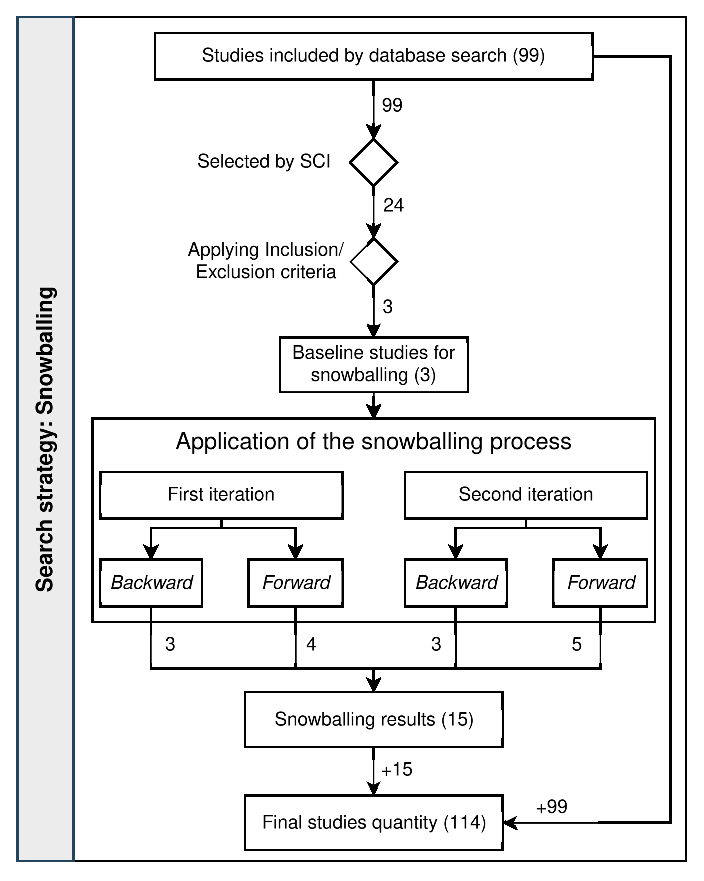
\includegraphics[scale=0.7]{resources/figures/sms-Snowball.eps}
	\caption{Snowball search strategy.}
	\label{figure:Snowball}
\end{figure}

This activity was conducted through Google Scholar and following the practice in the study~\cite{Ali-01}. The result obtained was \snowballNewStudies{} new studies. It should be noted that what is presented in this section and in Figure~\ref{figure:Snowball} is a representative summary of the snowball process, however, steps that were performed but do not contribute to the study objective are omitted.

% -------- Table : Inclusion/exclusion criteria ------------
\begin{table}
	\tbl{Inclusion/exclusion criteria}
	{
	\begin{tabular}{p{1.5cm}p{2.2cm}p{3.9cm}} \toprule
		\textbf{Category}         & \textbf{Inclusion} & \textbf{Exclusion}                                                                                             \\
		\midrule
		\textbf{Publication type} & Research articles  & Theses, book chapters, books, journals, conferences, and everything else not in the inclusive publication type \\
		\textbf{Period}           & From 2020 to 2024  & -                                                                                                              \\
		\textbf{Language}         & English            & -                                                                                                              \\
		\bottomrule
	\end{tabular}}
	\label{table:inclusion_exclusion_criteria}
\end{table}
% --------------------------------------------------------------
